\documentclass[conference,a4paper,10pt,onecolumn]{IEEEtran}

\usepackage{url}
\usepackage{listings}
\usepackage{subfigure}
\usepackage{multirow}
\usepackage{pictexwd}
\usepackage[absolute]{textpos}
\usepackage[english]{babel}
\usepackage{footnote}
\usepackage{graphicx}
   
\lstset{%
  keywordstyle=\bfseries,
  aboveskip=15pt,
  belowskip=15pt,
  captionpos=b,
  identifierstyle=\ttfamily,
  escapeinside={(*@}{@*)},
  stringstyle=\ttfamiliy,
  %frame=single,
  numbers=left, basicstyle=\scriptsize, numberstyle=\tiny, stepnumber=0, numbersep=2pt}

\newcommand{\prg}[3][tbp]{
\begin{figure}[#1]
  \lstinputlisting[language=C,keywordstyle=\bfseries,
  aboveskip=15pt,
  belowskip=15pt,
  captionpos=b,
  identifierstyle=\ttfamily,
  escapeinside={(*@}{@*)},
  stringstyle=\ttfamiliy,
  frame=single,
  numbers=left, basicstyle=\tiny, numberstyle=\tiny, stepnumber=0, numbersep=2pt]{fig/#2.cc}
  \caption{#3}
  \label{prg:#2}
\end{figure}
}

\newcommand{\prgFull}[3][tbp]{
  \lstinputlisting[language=C,keywordstyle=\bfseries,
  aboveskip=15pt, 
  belowskip=15pt,
  captionpos=b,
  identifierstyle=\ttfamily,
  escapeinside={(*@}{@*)},
  stringstyle=\ttfamiliy,
  %frame=tbrl,
  numbers=left, basicstyle=\tiny, numberstyle=\tiny, stepnumber=0, numbersep=2pt]{fig/#2.cc}
}


\newcommand{\tab}[3][ph]{
  \begin{table}[#1]
    {\centering\small\textsf{\input{fig/#2.tab}}\par}
    \caption{#3}
  \label{tab:#2}
  \end{table}
}

\newcommand{\fig}[4][ht!]{
  \begin{figure}[#1]
    {\centering{\includegraphics[#4]{fig/#2}}\par}
    \caption{#3}
    \label{fig:#2}
  \end{figure}
}


\newcommand{\Fig}[4][hp]{
  \begin{figure*}[#1]
    {\centering{\includegraphics[#4]{fig/#2}}\par}
    \caption{#3}
    \label{fig:#2}
  \end{figure*}
}

\def\sharedaffiliation{%
\end{tabular}
\begin{tabular}{cc}}
	
\hyphenation{sche-du-ling}

\begin{document}

\title{Towards a shared-data-aware multicore real-time scheduler\\}


\author{Giovani Gracioli and Ant\^{o}nio Augusto Fr\"{o}hlich\\
Federal University of Santa Catarina, Florian\'{o}polis, Brazil\\
\{giovani,guto\}@lisha.ufsc.br
}


\maketitle

\section{The Problem}

Multicore processors have been established in the multicore embedded real-time system domain. Several applications that used to be implemented in dedicated hardware, such as digital signal processing algorithms and baseband processing in wireless communication, can now be ported to software with similar performance and more support flexibility for developers (e.g., bug fixes, online updating, maintainability)~\cite{Cho2006}. Such applications process a considerable amount of data under real-time conditions and are composed of several real-time cooperating threads (threads that share data and run concurrently in the available cores). In this scenario, due to multicore processor organization, we must consider some important characteristics, specifically, the memory hierarchy~\cite{Zhuravlev:2010}. The memory hierarchy holds an important role, because it affects the estimation of the Worst-Case Execution Time (WCET), which is extremely important in the sense of guaranteeing that all threads will meet their deadlines through the design phase evaluation (schedulability analysis)~\cite{Marwedel2005,Suhendra2008}.

Several works have been proposed to deal with memory organization in multicore architectures and provide real-time guarantees~\cite{Cho2006,Anderson2008}. However, they only consider scenarios in which threads are independent (without data sharing). In this case, the influence among threads (contention for cache space and interference in the cache lines) can be solved by memory partitioning/locking mechanisms provided by a special hardware~\cite{Suhendra2008} or implemented into the real-time scheduler~\cite{Zhuravlev:2010,Guan2009}. 

The problem we are addressing in this paper rises from the memory hierarchy present in today's SMP architectures and their memory coherence protocols (e.g., MESI, MOESI, or MESIF). Each core has its own data and uses its private data cache for speeding up processing. However, when cores share data, each copy of the data is placed in the core's private cache and the cache-coherence protocol is responsible for keeping the consistency among copies (through bus snooping). When a core writes into a data that other cores have cached, the cache-coherence protocol invalidates all copies, causing an implicit delay in the application's execution time. In the same way, when a core reads a shared data that was just written by another core, the cache-coherence protocol does not return the data until it finds the cache that has the data, annotates that cache line to indicate that it is shared, and recovers the data to the reading core. These operations are performed automatically by the memory controller hardware and take hundreds of cycles (about the same time as accessing the off-chip RAM), increasing the application's execution time which may lead to deadline losses~\cite{BoydWickizer:10}. Two kinds of scaling problems occur due to shared memory contention~\cite{BoydWickizer:10}: access serialization to the same cache line done by the cache coherence protocol, which prevents parallel speedup, and saturation into the inter-core interconnection, also preventing parallel processing gains.

\section{Open Questions}
\label{sec:open}

Based on the problem description, we have identified the following open questions:

\begin{itemize}
	\item \textit{Task model.}  Traditional real-time task models do not take into account the parallelism and data dependencies presented in multicore processors. The parallel synchronous task model is an important step towards formally defining a task model for parallel real-time tasks~\cite{Saifullah:2011}. However, the task model presents restrictions and supports only DM and EDF scheduling policies. Moreover, is the parallel synchronous task model adequate for the described problem? We believe that there is a need for better parallel task models.
	\item \textit{Cache contention.} Are there techniques to reduce the contention for cache spaces and decrease the influence of the cache coherency protocols in applications that share data without relying on hardware redesign? Cache partitioning/locking techniques may be the answer for eliminating the contention for cache spaces. Partitioning/Locking isolates application workloads that interfere with each other, increasing the predictability. Nevertheless, when there is data sharing between parallel threads, cache partitioning does not solve the problem, because threads will access the same data location on the memory hierarchy. Moreover, what is the influence of partitioning on global, partitioned, and semi-partitioned real-time schedulers? There is still room for combining cache partitioning with other techniques to provide real-time guarantees for data sharing application.
	\item \textit{Real-time scheduling.} To the best of our knowledge, there is no shared-cache-aware real-time scheduler proposed in the literature. We believe that a shared-cache-aware real-time scheduler may benefit from static information collected by offline analyzers and run-time information collected by the hardware support, such as hardware performance counters (HPCs). However, which static information must be collected and which hardware events are more suitable for the scheduler are still open questions. Moreover, which techniques could the scheduler use to decrease the contention for shared data? For example, the scheduler can prevent a thread from being run to avoid the contention, but how about the real-time guarantees? How much time can a thread wait? Also, the schedulability tests must not be too pessimistic, such as the very pessimistic Global-EDF sufficient tests.
\end{itemize}

\section{Envisioned Solution Statement} 

Towards a solution for the problem, we envision a set of OS techniques designed to provide predictability and real-time guarantees for embedded multicore real-time applications. The proposed architecture is depicted in Figure~\ref{fig:proposed_solution} and is a step forward to mitigate the effects of contention for shared cache memory. It is composed of a two-level OS cache partitioning to minimize the contention for cache space between different applications (inter-application partitioning) and between threads of the same application (intra-application partitioning). It also has a shared memory-aware scheduler responsible for detecting and minimizing the influence of memory coherence from threads that share data (e.g., access serialization to the same cache line and saturation in the inter-core interconnection), while still compromising with real-time guarantees. 

\begin{figure}[ht]
\begin{minipage}[b]{0.45\linewidth}
\centering
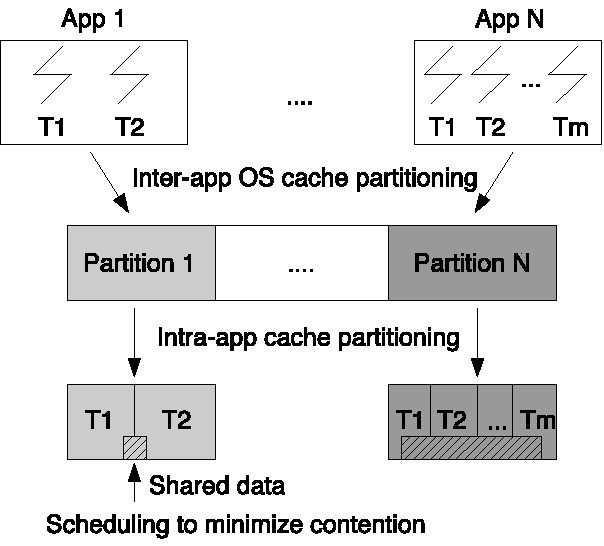
\includegraphics[scale=.48]{fig/proposed_solution.pdf}
\caption{Proposed envisioned solution architecture.}
\label{fig:proposed_solution}
\end{minipage}
\hspace{0.5cm}
\begin{minipage}[b]{0.45\linewidth}
\centering
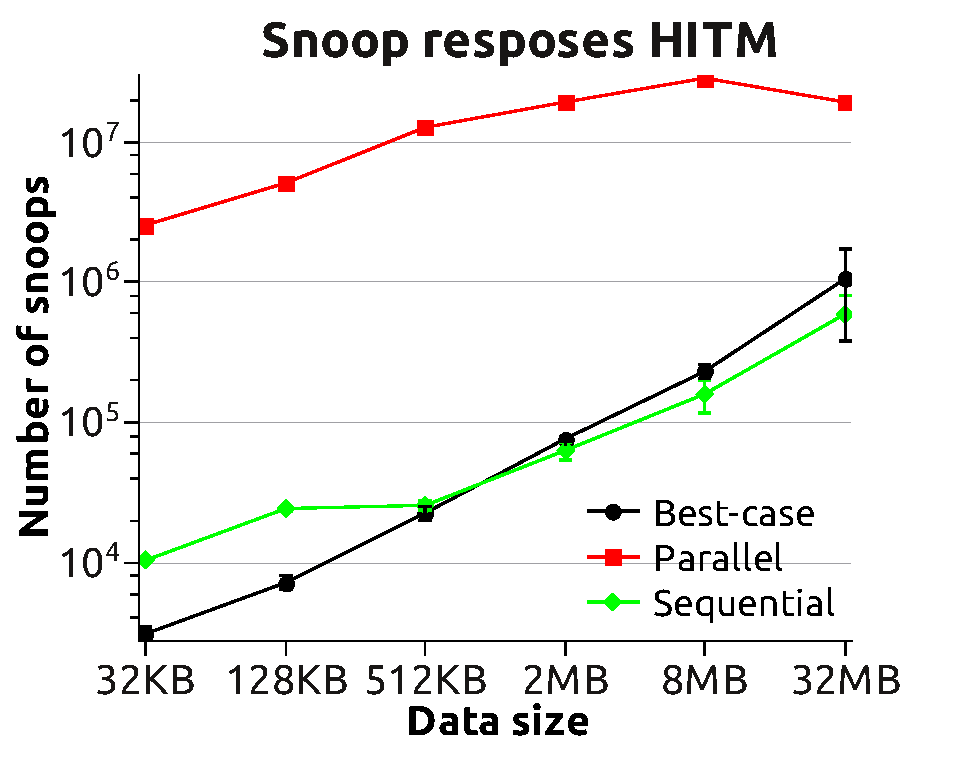
\includegraphics[scale=.35]{fig/HPC_ext_snoop_hitm2.pdf}
\caption{HPCs evaluation on Intel Q9550 processor: snoops HITM.}
\label{fig:HPC_ext_snoop_hitm2}
\end{minipage}
\end{figure}

We are currently investigating which hardware events can be used together with the scheduler and which techniques the scheduler could use to mitigate the cache coherency effects. For example, in an experiment carried out using the Intel Q9550, we measured the number of snoop requests in a synthetic benchmark. Figure~\ref{fig:HPC_ext_snoop_hitm2} shows the obtained results. We can note that the parallel application (in which there is data sharing) presents up to three orders of magnitude more snoop requests than the other two applications that do not share data. This experiment shows the feasibility of HPCs: they could correctly feed the scheduler with run-time information. The RTOS can use HPCs to detect sharing patterns among threads and take a scheduling decision, such as stopping a thread for a short period by sending an Inter-Processor Interrupt (IPI). We are also improving the multicore real-time support on the EPOS RTOS~\cite{Gracioli:2013}.

\section{Summary}
\label{sec:conc}

In this position paper we presented the problem of scheduling real-time threads considering data sharing and the implicit delay caused by the cache coherency protocols implemented on today's SMP processors. Our proposal towards a solution is a combination of OS techniques to alleviate the effects of the shared cache coherency. As future work, we intend to investigate techniques to be incorporated into the OS real-time scheduling and evaluate our proposed solution. Moreover, there are still relevant open questions, as described in Section~\ref{sec:open}. \footnotesize{This work was partially supported by the Coordination for Improvement of Higher Level Personnel (CAPES) grant, projects RH-TVD 006/2008 and 240/2008, and CAPES-DFAIT 004/2011.}

% references section
\bibliographystyle{IEEEtran}
\bibliography{references}

% that's all folks
\end{document}
